\documentclass[a4paper]{article}
\usepackage[english]{babel}
\usepackage[top=0.1in, left=1.1in, right=2.4in, bottom=0.1in]{geometry}
\usepackage{graphicx,color}
\usepackage{ragged2e}
\definecolor{orange}{RGB}{255,97,0}
\definecolor{blue}{RGB}{68,90,111}
\definecolor{hintergrund}{rgb}{0.99,0.99,0.99}
\pagecolor{hintergrund}
\renewcommand{\baselinestretch}{1}
\usepackage{fontspec}
\setmainfont[Mapping=text-tex]{Lato Light}

% Additional packages for subfigures and landscape mode
\usepackage{subcaption}
\usepackage{rotating}
\usepackage{lscape}

\begin{document}
\begin{sidewaysfigure}[htbp]
  \centering
  \begin{subfigure}[b]{0.45\linewidth}
    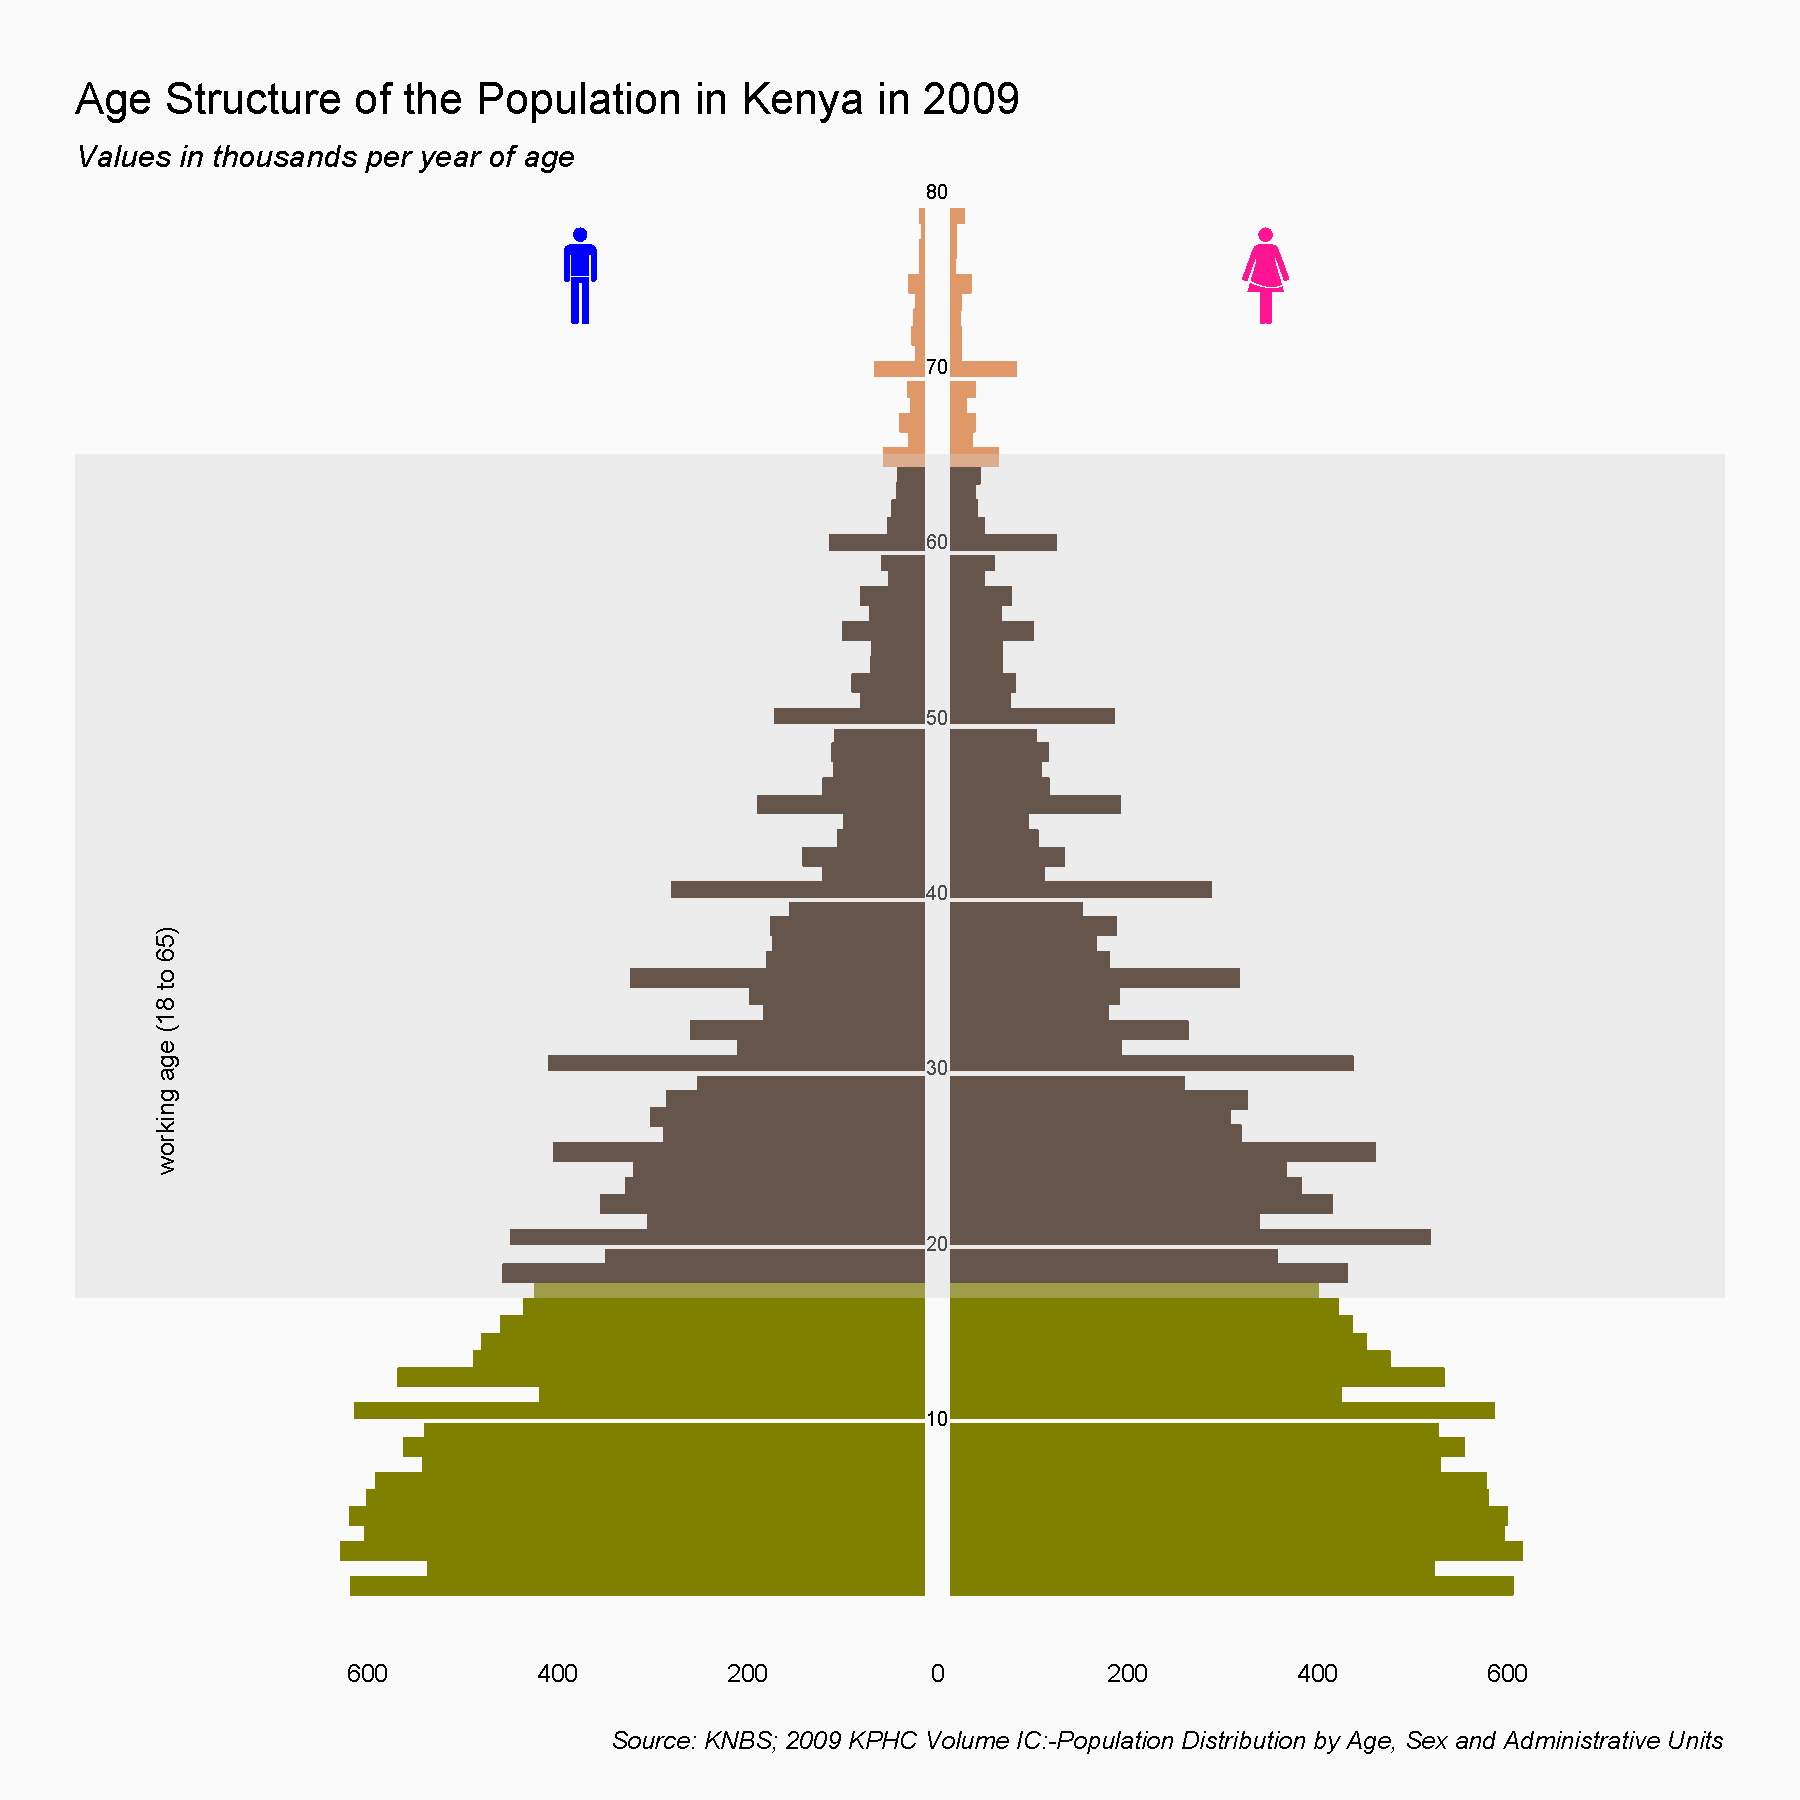
\includegraphics[width=\linewidth]{Kenyan_Population_2009.pdf}
    \caption{\centering KPHC 2009}
    \label{fig:Population distribution by age and sex 2009}
  \end{subfigure}
  \hfill
  \begin{subfigure}[b]{0.45\linewidth}
    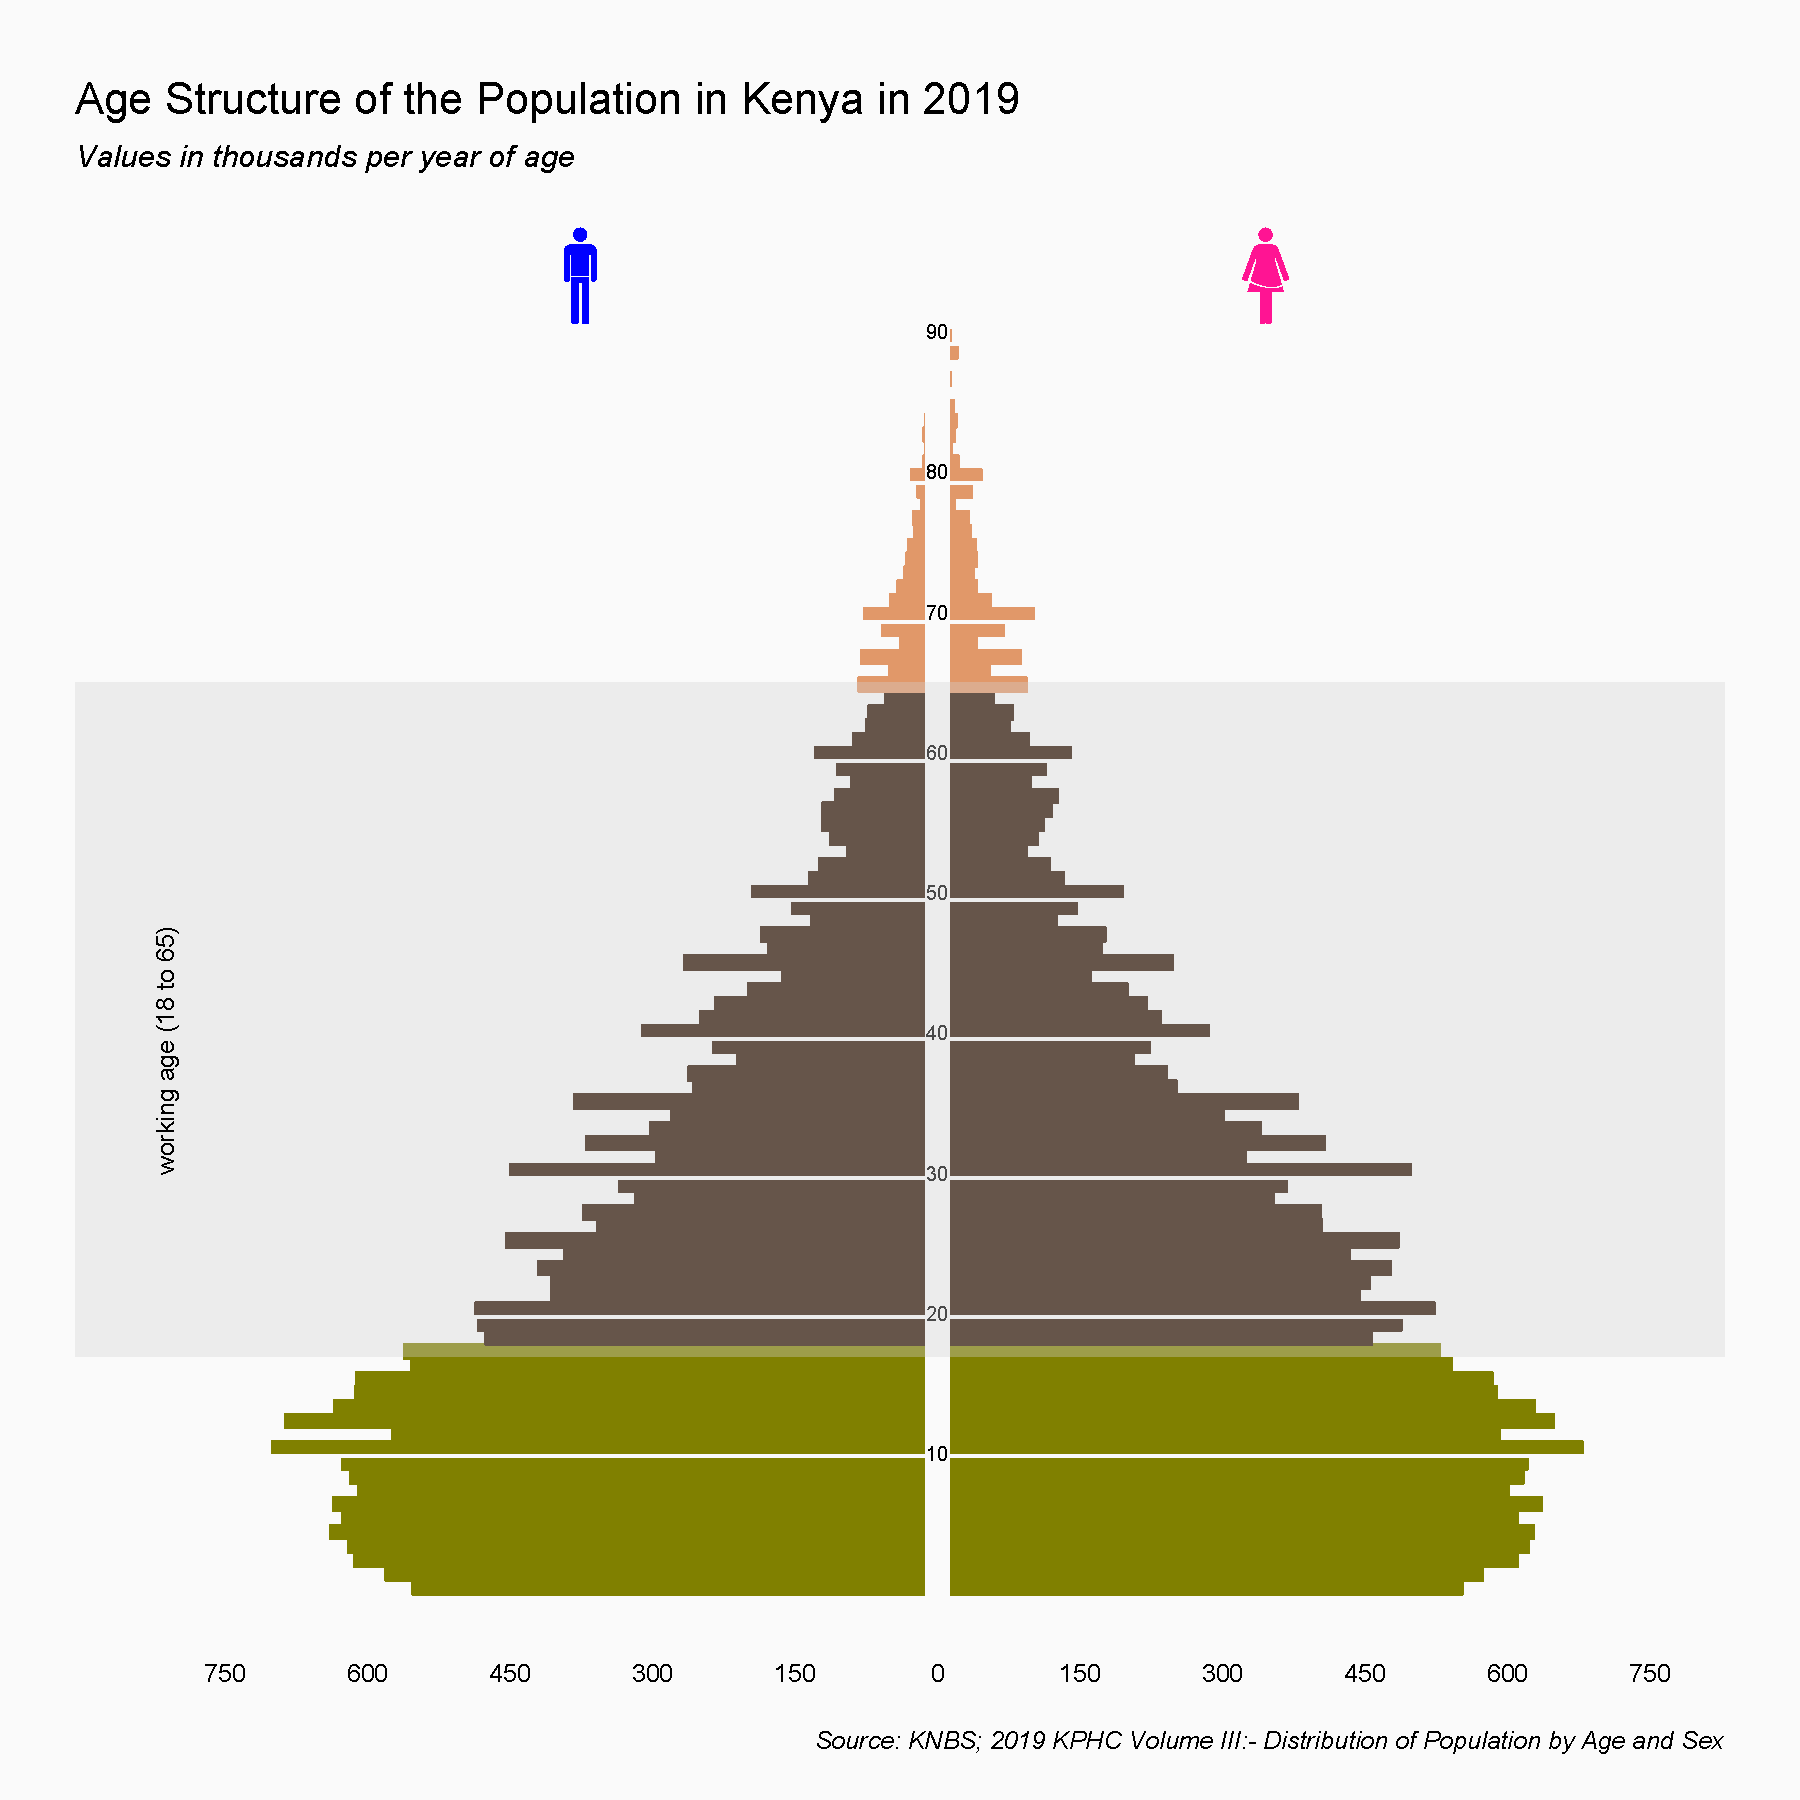
\includegraphics[width=\linewidth]{Kenyan_Population_2019.pdf}
    \caption{\centering KPHC 2019}
    \label{fig:Population distribution by age and sex 2019}
  \end{subfigure}
  \caption{Population distribution by age and sex in Kenya: KPHC 2009 and KPHC 2019}
  \label{fig:KPHC comparison}
  \vspace{1em}
  \centering
  \textbf{Author:} Mr. Muia, Kelvin Mwaka \\
  \textbf{Note:} The data used in these visuals was scrapped from publications by the Kenya National Bureau of Statistics for the Kenyan Population and Housing Census (KPHC) of 2009 \& 2019.
\end{sidewaysfigure}

\end{document}
